\DiaryEntry{Volumes of high-dimensional Unit Ball and Unit Box}{2018-04-11}{Maths}

We define a unit ball $\Sc_N$ as the following $N$-dimensional set

\bee
\Sc_N = \{x\in \mR^N | |x|^2 < 1\}
\eee

where $|\cdot|$ is the normal $2$-norm. According to \href{https://en.wikipedia.org/wiki/Volume_of_an_n-ball}{Wikipedia}, the volume of such a ball is given by

\bee
V(\Sc_N) = \frac{\pi^{N/2}}{\Gamma(N/2+1)}
\eee

A unit box $\Bc_N$ is defined as the $N$-dimensional set

\bee
\Bc_N = \{x \in \mR^N | x_i \in [-1,1]\}
\eee

with volume

\bee
V(\Bc_N) = 2^N
\eee

Suppose we generate random points in the unit box uniformly and ask for the probability with which these points are contained in the unit ball. This probability is given by the ratio of the two volumes; i.e.

\todo{check formula and plot}
\bee
\frac{\pi^{N/2}}{2^N \Gamma(N/2+1)}
\eee

The following Figure shows this ratio.

\begin{figure}[H]
	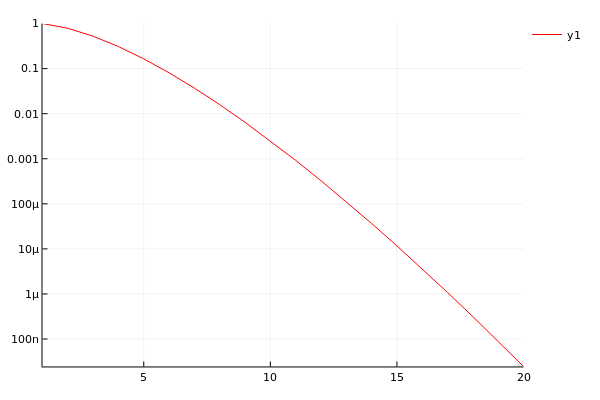
\includegraphics[scale=0.7]{images/high_dim_02_01.png}
\end{figure}

\paragraph{Intuition.} The ball touches the sides of the box at $2N$ positions, but there are many more corners, namely $2^N$. The distance between the corners deserves some more attention. Consider two corner points of the unit cube $p_1, p_2$. Each component of the point can have the value $\pm 1$. The shortest diagonal is when the points differ in two coordinates; e.g.

\bee
p_1=[-1,1,1], \quad p_2 = [1,-1,1]
\eee

and the distance is $\sqrt{2}2$. The longest diagonal is when all coordinates are different; e.g.

\bee
p_1=[-1,1,-1], \quad p_2 = [1,-1,1]
\eee

and is $\sqrt{3}2$ and in the general case of $N$ dimensions $\sqrt{N}2$. This expression grows with $N$: Although the length of the unit cube is fixed (length $2$), the diagonals increase unbounded with $N$. If our random points are located uniformly inside the unit cube, the probability that they located "near" the corners instead near the center becomes increasingly large. This is the reason why the probability for the points to lie within the unit ball becomes zero.


